\documentclass[dvipdfmx,cjk]{beamer}
%\usepackage{bxdpx-beamer}% dvipdfmxなので必要
%\usepackage{pxjahyper}% 日本語で'しおり'したい
%\documentclass[ckj]{beamer}
%\usepackage{etex}
%\usetheme{Warsaw}
\usetheme{Malmoe}
%\usetheme{AnnArbor}
%\usetheme{Hannover}
%\usetheme{Bergen}
%\usetheme{Berlin}
%\usetheme{Singapore}
%\usetheme{Montpellier}
%\usetheme{Pittsburgh}
\usepackage{graphicx}
\usepackage{latexsym,amssymb}
%\usepackage{epsbox}
%\usepackage{multirow}
\usepackage{fancybox}
\usepackage{fancyvrb}
%\usepackage{listings}
\usepackage{tabularx}
%\usepackage{pstricks,pst-node,pst-tree}
%\usepackage{multimedia}
%\usepackage{pstricks,pst-node,pst-tree}
%\usepackage{pst-all}
\usepackage{tikz}
\usetikzlibrary{calc}
\usepackage{ascmac}
\usepackage{ulem}
\usepackage{listings}
\lstloadlanguages{C,LLVM}
%\usepackage{color,soul}
%\include{prooftree}
%\lstloadlanguages{pascal}
\renewcommand{\kanjifamilydefault}{\gtdefault}
\renewcommand{\familydefault}{\sfdefault}

\newcommand{\greentext}[1]{{\color[rgb]{0,0.5,0}{#1}}}
\newcommand{\redtext}[1]{{\color[rgb]{0.8,0,0}{#1}}}
\newcommand{\bluetext}[1]{{\color[rgb]{0,0,0.8}{#1}}}

\newcommand{\tuple}[1]{\langle{#1}\rangle}

\newcommand{\First}{\mathsf{First}_1}
\newcommand{\Follow}{\mathsf{Follow}_1}

%%pdt simulation

\newcommand{\pdtline}[6]{%
    \uncover<#6->{
        \node at (${#5}*(0,-.3)+(0,.3)$) {$\vdash$};%
        \node at (${#5}*(0,-.3)+(1.5,.3)$) {\parbox{12em}{(#1,}};%
        \node at (${#5}*(0,-.3)+(4.5,.3)$) {\parbox{10em}{#2,}};%
        \node at (${#5}*(0,-.3)+(5.7,.3)$) {\parbox{10em}{#3)}};%
        \node at (${#5}*(0,-.3)+(8,.3)$) {\parbox{20em}{#4}};%
    }
}

\newcommand{\initpdtline}[6]{%
    \uncover<#6->{
        \node at (${#5}*(0,-.3)+(1.5,.3)$) {\parbox{12em}{(#1,}};%
        \node at (${#5}*(0,-.3)+(4.5,.3)$) {\parbox{10em}{#2,}};%
        \node at (${#5}*(0,-.3)+(5.7,.3)$) {\parbox{10em}{#3)}};%
        \node at (${#5}*(0,-.3)+(8,.3)$) {\parbox{20em}{#4}};%
    }
}

\newtheorem{Def}{定義}
\newtheorem{Lem}{補題}
\newtheorem{Thm}{定理}
\newtheorem{Prop}{命題}

\definecolor{lightlightgrey}{rgb}{0.95,0.95,0.95}

\newcommand{\ttpl}{\texttt{+}}
\newcommand{\ttsb}{\texttt{-}}
\newcommand{\ttmu}{\texttt{*}}
\newcommand{\ttdv}{\texttt{/}}
\newcommand{\tteq}{\texttt{=}}




%\newcommand{\greentext}[1]{{\color[rgb]{0,0.5,0}{#1}}}
%\newcommand{\redtext}[1]{{\color[rgb]{0.8,0,0}{#1}}}

\newcommand{\lecturedate}{2026/10/23}

\newcommand{\ttlp}{{\tt (}}
\newcommand{\ttrp}{{\tt )}}
\newcommand{\makenewlabel}{{\tt newLabel}()}
\newcommand{\genlabel}[1]{{\tt generate}(`{\tt label}\ {#1}')}
\newcommand{\genifnot}[2]{{\tt generate}(`{\tt if\_not}\ {#1}\ {\tt goto}\ {#2})'}
\newcommand{\gengoto}[1]{{\tt generate}(`{\tt goto}\ {#1}')}

\graphicspath{{figs261023/}}

\cornersize{0.25}

\setbeamertemplate{frametitle}[default][center]
\setbeamertemplate{footline}{\hfill
コンパイラ\quad\lecturedate
\hfill\insertframenumber/\inserttotalframenumber\hspace*{1zw}}
\newcounter{coffee}
\setbeamercovered{transparent=10}
\title{コンパイラ(7)}
\date{\lecturedate}
\begin{document}
\frame{\titlepage}

\section{中間コード生成}

\subsection{中間コード}

\begin{frame}
  \frametitle{抽象構文}

  \[\textsf{ID}\tteq\textsf{ID}\ttmu\ttlp\textsf{ID}\ttpl\textsf{ID}\ttrp\]

  \begin{tabularx}{\textwidth}{m{.4\textwidth}m{.2\textwidth}m{.3\textwidth}}
    \begin{minipage}{.4\textwidth}
      \[\begin{array}{rcl}
          E & \rightarrow & E\ \ttpl\ T           \\
          E & \rightarrow & T                     \\
          T & \rightarrow & T\ \ttmu\ F           \\
          T & \rightarrow & F                     \\
          F & \rightarrow & \textsf{ID}           \\
          F & \rightarrow & \ttlp\ E\ \ttrp       \\
          S & \rightarrow & \textsf{ID}\ \tteq\ E
        \end{array}
      \]
    \end{minipage}                      &
    \begin{minipage}{.4\textwidth}
      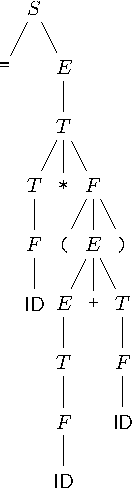
\includegraphics[scale=0.5]{concParseTree-crop.pdf}
    \end{minipage} &
    \[\begin{array}{rcl}
          E & \rightarrow & E\ \ttpl\ E           \\
          E & \rightarrow & E\ \ttmu\ E           \\
          E & \rightarrow & \textsf{ID}           \\
          S & \rightarrow & \textsf{ID}\ \tteq\ E
        \end{array}
    \]                                                    \\[3cm]
    \multicolumn{2}{c}{具体構文および構文木}                      &
    抽象構文
  \end{tabularx}
  \begin{center}
    \greentext{抽象構文：具体構文から意味に関わる部分を抽出}
  \end{center}
\end{frame}

\begin{frame}
  \frametitle{抽象構文木}
  解析木からコード生成に必要な部分を残して変形したもの\\[10pt]
  \greentext{内部接点=演算子、葉=オペランド}

  \vspace*{1zw}

  構文主導型変換によって中間コードを生成する際に便利

  \vspace*{1zw}

  等価な意味を持つ抽象構文木=最適化に利用

  \vspace*{10pt}

  \begin{tabular}{ccc}
    \scalebox{0.75}{
      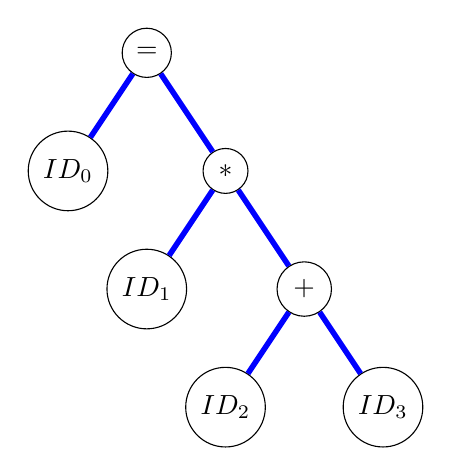
\begin{tikzpicture}
        \node[draw,circle] (N0) at (1,4.5) {$=$};
        \node[draw,circle] (N1) at (0,3) {$ID_0$};
        \node[draw,circle] (N2) at (2,3) {$\ast$};
        \node[draw,circle] (N3) at (1,1.5) {$ID_1$};
        \node[draw,circle] (N4) at (3,1.5) {$+$};
        \node[draw,circle] (N5) at (2,0) {$ID_2$};
        \node[draw,circle] (N6) at (4,0) {$ID_3$};
        \path[-,color=blue,line width=2pt] (N0) edge (N1)
        (N0) edge (N2)  (N2) edge (N3)
        (N2) edge (N4)  (N4) edge (N5)
        (N4) edge (N6);
      \end{tikzpicture}
    } & \quad &
    \scalebox{0.75}{
      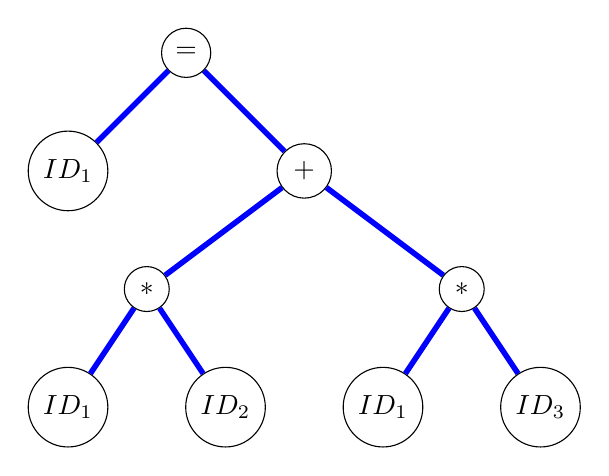
\begin{tikzpicture}
        \node[draw,circle] (N0) at (1.5,4.5) {$=$};
        \node[draw,circle] (N1) at (0,3) {$ID_1$};
        \node[draw,circle] (N2) at (3,3) {$+$};
        \node[draw,circle] (N3) at (1,1.5) {$\ast$};
        \node[draw,circle] (N4) at (5,1.5) {$\ast$};
        \node[draw,circle] (N5) at (0,0) {$ID_1$};
        \node[draw,circle] (N6) at (2,0) {$ID_2$};
        \node[draw,circle] (N7) at (4,0) {$ID_1$};
        \node[draw,circle] (N8) at (6,0) {$ID_3$};
        \path[-,color=blue,line width=2pt]
        (N0) edge (N1)  (N0) edge (N2)
        (N2) edge (N3)  (N2) edge (N4)
        (N3) edge (N5)  (N3) edge (N6)
        (N4) edge (N7)  (N4) edge (N8);
      \end{tikzpicture}

    }
  \end{tabular}
\end{frame}

\begin{frame}
  \frametitle{逆ポーランド記法}
  \greentext{抽象構文木の後置記法}:
  スタックを用いた実行に対応

  \[
    \begin{array}{cccccccc}
      \begin{array}{|c|}
        \    \\\hline
        ID_0 \\\hline
      \end{array}
                                     & \rightarrow &
      \begin{array}{|c|}
        \    \\\hline
        ID_1 \\\hline
        ID_0 \\\hline
      \end{array}
                                     & \rightarrow &
      \begin{array}{|c|}
        \    \\\hline
        ID_2 \\\hline
        ID_1 \\\hline
        ID_0 \\\hline
      \end{array}
                                     & \rightarrow &
      \begin{array}{|c|}
        \    \\\hline
        ID_3 \\\hline
        ID_2 \\\hline
        ID_1 \\\hline
        ID_0 \\\hline
      \end{array}
                                     & \rightarrow
      \\
      \mbox{push $ID_0$}             &             &
      \mbox{push $ID_1$}             &             &
      \mbox{push $ID_2$}             &             &
      \mbox{push $ID_3$}                             \\
      \begin{array}{|c|}
        \                      \\\hline
        {\tiny val(ID_3*ID_2)} \\\hline
        ID_1                   \\\hline
        ID_0                   \\\hline
      \end{array}
                                     & \rightarrow &
      \multicolumn{3}{c}{
        \begin{array}{|c|}
          \                             \\\hline
          {\tiny val((ID_3*ID_2)+ID_1)} \\\hline
          ID_0                          \\\hline
        \end{array}}
                                     & \rightarrow &
      \begin{array}{|c|}
        \ \\\hline
      \end{array}                              \\
      \mbox{$*$}                     &             &
      \multicolumn{3}{c}{\mbox{$+$}} &             &
      \mbox{$=$}                                     \\
    \end{array}
  \]
\end{frame}

\begin{frame}
  \frametitle{3番地コード}
  \[
    \begin{array}{lp{.5\textwidth}}
      C = A\theta B & $+$,$-$,$*$,$/$,$\mathsf{and}$,$\mathsf{or}$,$>$,$>=$,$=$,$!=$,$<=$,$<$ \\[5pt]
      B = \theta A  & $-$,$\mathsf{not}$                                                      \\[5pt]
      B = A                                                                                   \\[5pt]
      \multicolumn{2}{l}{\mbox{\greentext{Jump on condition}}}                                \\[5pt]
      \multicolumn{2}{l}{\mathtt{if}\ A\ \mathtt{goto}\ L}                                    \\[5pt]
      \multicolumn{2}{l}{\mathtt{if}\ not A\ \mathtt{goto}\ L}                                \\[5pt]
      \multicolumn{2}{l}{\mbox{\greentext{Unconditional Jump}}}                               \\[5pt]
      \multicolumn{2}{l}{\mathtt{goto}\ L}
    \end{array}
  \]
\end{frame}

\begin{frame}
  \frametitle{抽象構文木からの３番地コード生成}
  \begin{tabularx}{\textwidth}{XX}
    \multicolumn{1}{m{.5\textwidth}}{
      \begin{tabularx}{.5\textwidth}{X}
        $ID_0=ID_1\ast(ID_2+ID_3)$ \\[25pt]
        $\begin{array}{l}
             \uncover<2->{t_1=ID_0}        \\
             \uncover<3->{t_3=ID_1}        \\
             \uncover<4->{t_5=ID_2}        \\
             \uncover<5->{t_6=ID_3}        \\
             \uncover<6->{t_4=t_5+t_6}     \\
             \uncover<7->{t_2=t_3\ast t_4} \\
             \uncover<8->{t_7=(t_1=t_6)}
           \end{array}$
      \end{tabularx}
    }
     &
    \multicolumn{1}{m{.4\textwidth}}{
      \scalebox{0.75}{
        \begin{tikzpicture}
          \node[draw,circle,label={135:{$t_0$}}] (N0) at (1,4.5) {$=$};
          \node[draw,circle,label={135:{$t_1$}}] (N1) at (0,3) {$ID_0$};
          \node[draw,circle,label={45:{$t_2$}}] (N2) at (2,3) {$\ast$};
          \node[draw,circle,label={135:{$t_3$}}] (N3) at (1,1.5) {$ID_1$};
          \node[draw,circle,label={45:{$t_4$}}] (N4) at (3,1.5) {$+$};
          \node[draw,circle,label={135:{$t_5$}}] (N5) at (2,0) {$ID_2$};
          \node[draw,circle,label={45:{$t_6$}}] (N6) at (4,0) {$ID_3$};
          \path[-,color=blue,line width=2pt] (N0) edge (N1)
          (N0) edge (N2)  (N2) edge (N3)
          (N2) edge (N4)  (N4) edge (N5)
          (N4) edge (N6);

          \only<2->{\draw[->,color=red,line width=2pt] (0.8,4.5) -- (-0.2,3.2);}
          \only<3->{\draw[color=red,line width=2pt] (0.2,2.8) to[in=180] (1,4);
            \draw[color=red,line width=2pt] (1,4) to[out=0,in=90] (1.6,3);
            \draw[->,color=red,line width=2pt] (1.6,3) to [out=270,in=60] (1,1.7);
          }
          \only<4->{\draw[color=red,line width=2pt] (1.2,1.7) to [in=180] (2,2.5);
            \draw[color=red,line width=2pt](2,2.5) to [out=0,in=90] (2.6,1.5);
            \draw[->,color=red,line width=2pt](2.6,1.5) to [out=270,in=60] (2,0.2);}
          \only<5->{\draw[color=red,line width=2pt] (2.2,0.2) to [in=180] (3,1);
            \draw[->,color=red,line width=2pt] (3,1) to [out=0,in=120] (3.7,0.2);}
          \only<6->{\draw[->,color=red,line width=2pt] (4,0.3) -- (3.3,1.3);}
          \only<7->{\draw[->,color=red,line width=2pt] (3,1.8) -- (2.2,2.8);}
          \only<8->{\draw[->,color=red,line width=2pt] (2,3.2) -- (1.3,4.5);}
        \end{tikzpicture}
      }}
  \end{tabularx}
  \begin{center}
    \only<1>{\greentext{抽象構文木に一時変数$t_i$を割り当てる}}
    \only<2>{\greentext{ポストオーダーでトレースし，$t_1=ID_0$を生成}}
    \only<3>{\greentext{ポストオーダーでトレースし，$t_3=ID_1$を生成}}
    \only<4>{\greentext{ポストオーダーでトレースし，$t_5=ID_2$を生成}}
    \only<5>{\greentext{ポストオーダーでトレースし，$t_6=ID_3$を生成}}
    \only<6>{\greentext{ポストオーダーでトレースし，$t_4=t_5 + t_6$を生成}}
    \only<7>{\greentext{ポストオーダーでトレースし，$t_2=t_3 \ast t_4$を生成}}
    \only<8>{\greentext{ポストオーダーでトレースし，$t_0=(t_1 = t_2)$を生成}}
  \end{center}
\end{frame}

% \begin{frame}
%  \frametitle{スタックマシンによる3番地コード}
%  $C=A\theta B$\\
%  逆ポーランド記法:$\mbox{push A},\mbox{push B},\theta$\\
%  \quad スタックトップを$C$に格納
%  \[
%  \begin{array}{cccccc}
%   \begin{array}{|c|}
%    \ \\\hline
%    A \\\hline
%   \end{array} & \rightarrow &
%   \begin{array}{|c|}
%    \ \\\hline
%    B \\\hline
%    A \\\hline
%   \end{array} & \rightarrow &
%   \begin{array}{|c|}
%    \ \\\hline
%    C \\\hline
%   \end{array} & \\
%   \mbox{push A} & & \mbox{push B} & & \multicolumn{2}{l}{\mbox{pop};\mbox{pop};\theta;\mbox{push C}}
%  \end{array}
%  \]

%  \begin{trivlist}
%    \item 単純に実行可能で抽象構文木をポストオーダーでトラバースすることで中間コード生成が可能。
%    \item 最適化のコストが大きい
%    \item スタックマシンの考え方に基づいて中間コードを生成する
%    \item 演算対象となるメモリを抽象的に指定する（静的単一代入）
%  \end{trivlist}
% % \begin{center}
% %  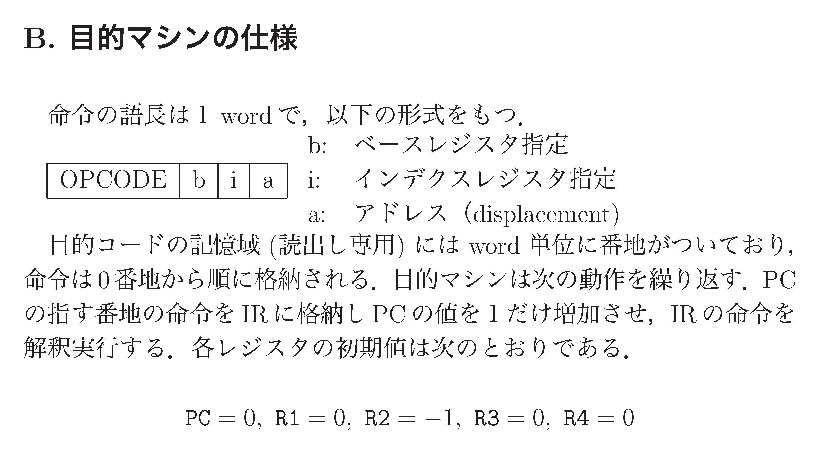
\includegraphics[scale=0.6]{inst00.eps}
% % \end{center}
% \end{frame}

\begin{frame}[fragile]
  \frametitle{手続き呼び出しの3番地コード}
  \begin{center}
    \begin{tabularx}{.9\textwidth}{XX}
      \multicolumn{1}{m{.4\textwidth}}{
        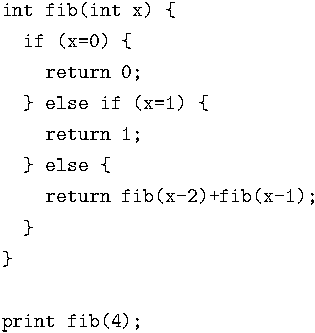
\includegraphics[scale=0.6]{fib_src-crop.pdf}
      }
       &
      \multicolumn{1}{m{.4\textwidth}}{
        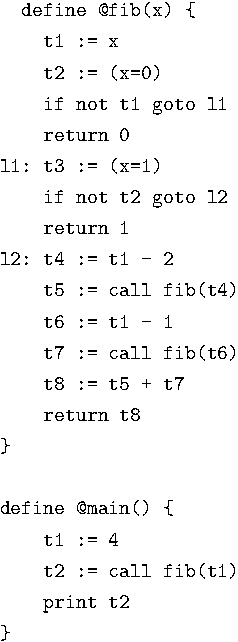
\includegraphics[height=0.75\textheight]{fib_3add-crop.pdf}
      }
    \end{tabularx}
  \end{center}
  {\small\color[rgb]{0,0.5,0}
  {\begin{tabular}{l}定義：\verb|define @|関数名(仮引数リスト) \\
      呼出：\verb|call @|関数名(実引数リスト)\end{tabular}}}
\end{frame}

% \begin{frame}[fragile]
% \frametitle{LLVM-IR}
% \begin{Verbatim}[fontsize=\scriptsize,label=HelloWorld.c,frame=single,numbers=left,numbersep=2pt]
% #include <stdio.h>
% int main() {
%   printf("HelloWorld\n");
%   return 0;
% }
% \end{Verbatim}

% \vspace*{5pt}

% \begin{Verbatim}[fontsize=\scriptsize,frame=single,showspaces=true]
% clang -emit-llvm -S -o HelloWorld.ll HelloWorld.c
% \end{Verbatim}

% \vspace*{5pt}

% \begin{Verbatim}[fontsize=\tiny,frame=single,label={\scriptsize HelloWorld.ll},numbers=left,numbersep=2pt]
% @.str = private unnamed_addr constant [13 x i8] c"Hello World\0A\00", align 1

% ; Function Attrs: noinline nounwind optnone ssp uwtable
% define i32 @main() #0 {
%   %1 = alloca i32, align 4
%   store i32 0, i32* %1, align 4
%   %2 = call i32 (i8*, ...) @printf(i8* getelementptr inbounds 
%                  ([13 x i8], [13 x i8]* @.str, i32 0, i32 0))
%   ret i32 0
% }

% declare i32 @printf(i8*, ...) #1
% \end{Verbatim}
% \end{frame}

%
%
%\begin{frame}
% \frametitle{演習コンパイラのコード}
% \only<1>{
% \begin{center}
%  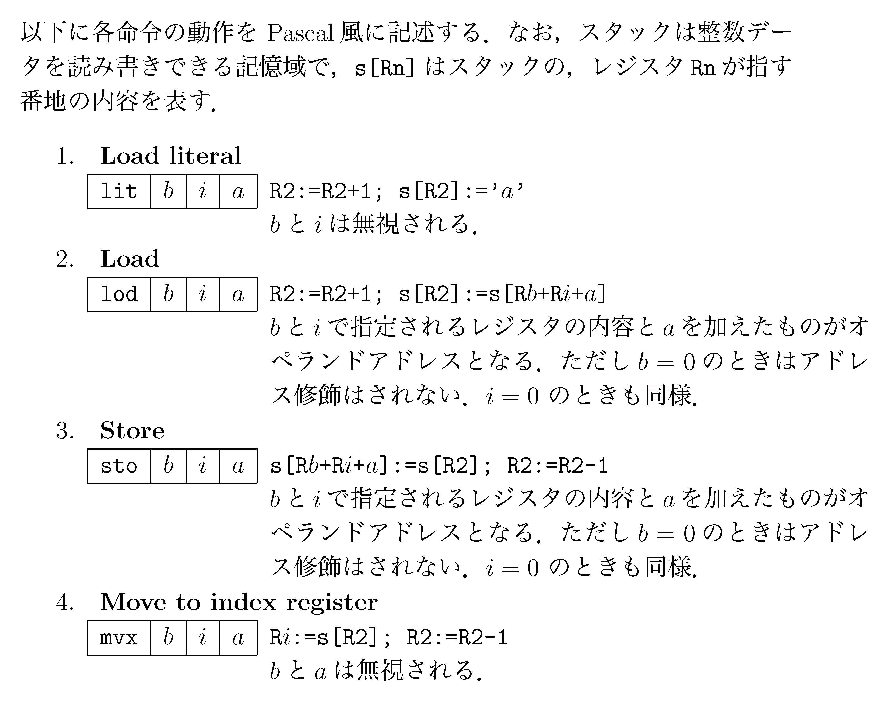
\includegraphics[scale=0.6]{inst01.eps}
% \end{center}
% }
% \only<2>{
% \begin{center}
%  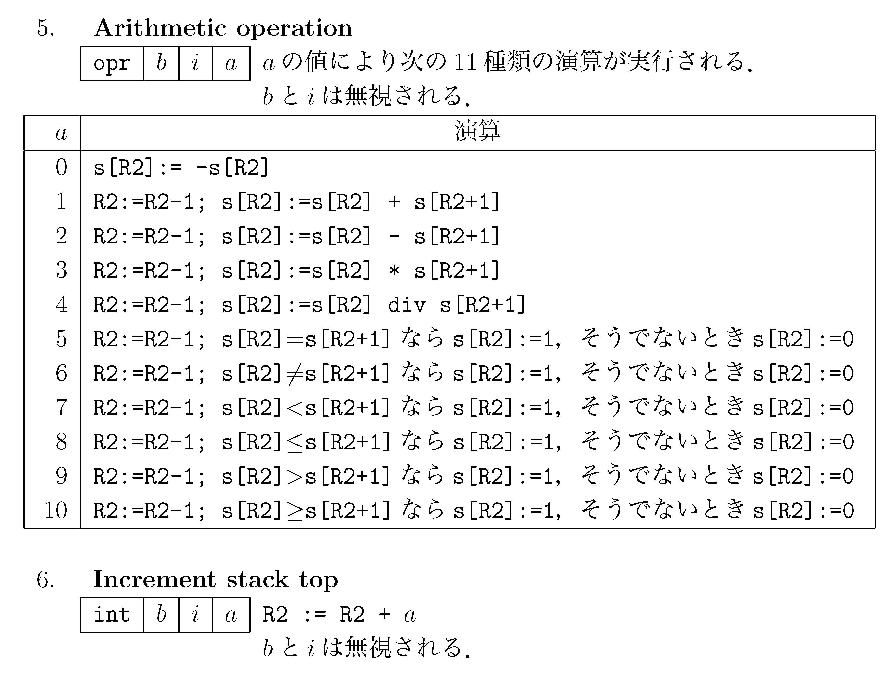
\includegraphics[scale=0.6]{inst02.eps}
% \end{center}
% }
% \only<3>{
% \begin{center}
%  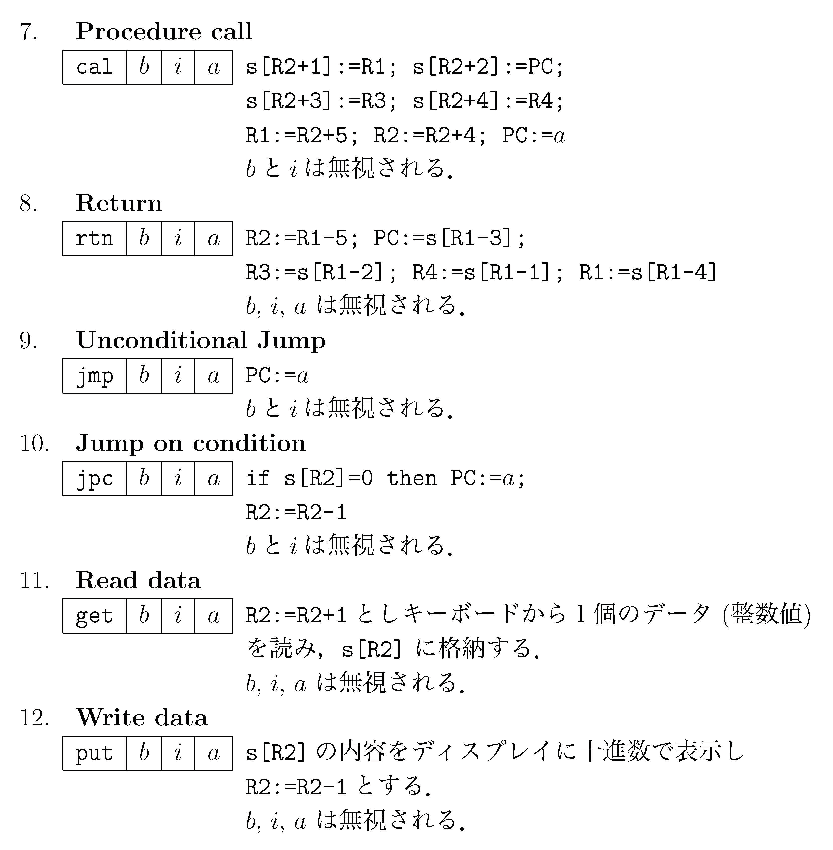
\includegraphics[scale=0.5]{inst03.eps}
% \end{center}
% }
%\end{frame}

% \begin{frame}
% \frametitle{LLVM-IRの命令\footnote{「きつねさんでもわかるLLVM」から引用}(メモリアクセス1)
% }
% {\scriptsize
% \begin{tabularx}{\textwidth}{|l|X|X|}\hline
% {\tt alloca} & 
%   result=alloca$\langle$type$\rangle$\newline
%     \quad [,$\langle$type$\rangle$ $\langle$NumElements$\rangle$]\newline
%     \quad [,align$\langle$alignment$\rangle$]
% & メモリ確保命令\newline type $\times$ NumElementsの領域を関数のスタックフレーム上に確保\\\hline
% {\tt load} & 
%   result=load [volatile]\newline
%   \quad $\langle$type$\rangle^\ast$ $\langle$pointer$\rangle$\newline
%   \quad [,align$\langle$alignment$\rangle$]\newline
%   \quad [,!nontemporal!$\langle$index$\rangle$]\newline
%   \quad [,!invariant.load !$\langle$index$\rangle$]\newline 
%   result=load atomic [volatile]\newline
%   \quad $\langle$type$\rangle^\ast$ $\langle$pointer$\rangle$\newline
%   \quad $\langle$singlethread$\rangle$ $\langle$ordering$\rangle$\newline
%   !index=! i32 1\newline
%   \quad align $\langle$alignment$\rangle$
% & ロード命令\newline
%     pointerが指すメモリアドレスから値を読み出す\newline
%     volatileが指定されている場合、最適化はload命令の実行順や実行数をほかのvolatileな命令に変更することができない\\\hline
% \end{tabularx}
% }
% \end{frame}

% \begin{frame}{LLVM-IRの命令(メモリアクセス2)}

% {\scriptsize 
% \begin{tabularx}{\textwidth}{|l|X|X|}\hline
% {\tt store} &
%   store [volatile]\newline
%   \quad $\langle$type$\rangle$ $\langle$value$\rangle$\newline
%   \quad $\langle$type$\rangle^\ast$ $\langle$pointer$\rangle$\newline
%   \quad [,align $\langle$alignment$\rangle$]\newline
%   \quad [,!nontemporal !$\langle$index$\rangle$]\newline
%   store atomic [volatile]\newline
%   \quad $\langle$type$\rangle$ $\langle$value$\rangle$\newline
%   \quad $\langle$type$\rangle^\ast$ $\langle$pointer$\rangle$\newline
%   \quad [singlethread] $\langle$ordering$\rangle$\newline
%   \quad align $\langle$alignment$\rangle$
%   & ストア命令\newline poinerが指すメモリアドレスに値を格納する\newline volatileが指定されている場合、最適化はstore命令の実行順や実行数をほかのvolatileな命令に変更することができない\\\hline
%   {\tt getelementptr} &
%   result = getelemntptr\newline
%   \quad $\langle$ptyple$\rangle^\ast$ $\langle$ptrval$\rangle$\newline
%   \quad \{, $\langle$type$\rangle$ $\langle$idx$\rangle$ \}$^\ast$\newline
%   result = getelementptr inbounds\newline
%   \quad $\langle$ptyple$\rangle^\ast$ $\langle$ptrval$\rangle$\newline
%   \quad \{, $\langle$type$\rangle$ $\langle$idx$\rangle$ \}$^\ast$\newline
%   result = getelementptr\newline
%   \quad $\langle$ptr vector$\rangle$,\newline
%   \quad $\langle$vector index type$\rangle$ $\langle$idex$\rangle$
%   &
%   要素アドレス取得命令\newline
%   合成型内の要素のアドレスを計算する\newline
%   prtvalが指す青dレスをベースとしてidxで指定したインデックスの要素アドレスを計算する\\\hline
% \end{tabularx}
% }
% \end{frame}

% \begin{frame}
% \frametitle{LLVM-IRの命令(演算命令)}
% {\scriptsize
% \begin{tabularx}{\textwidth}{|l|X|X|}\hline
% {\tt add} & {\tiny
% result = add $\langle$type$\rangle$ $\langle$op1$\rangle$ $\langle$op2$\rangle$	\newline
% result = add nuw $\langle$type$\rangle$ $\langle$op1$\rangle$ $\langle$op2$\rangle$	\newline
% result = add nsw $\langle$type$\rangle$ $\langle$op1$\rangle$ $\langle$op2$\rangle$	\newline
% result = add nuw nsw $\langle$type$\rangle$ $\langle$op1$\rangle$ $\langle$op2$\rangle$}
% &
% 加算命令\newline op1とop2を加算して結果を返す。op1, op2は整数か整数のベクタ。\newline
% nuw = No Unsigned Wrap, nsw = No Signed Wrap/ オーバーフローが発生したときに結果が未定義\\\hline
% \end{tabularx}
% }

% \vspace*{10pt}

% 同様な演算命令 fadd, sub, fsub, mul, fmul, udiv, sdiv, fdiv, urem,srem,frem(剰余)
% \end{frame}

% \begin{frame}
% \frametitle{LLVM-IRの命令(制御命令)}
% {\scriptsize
% \begin{tabularx}{\textwidth}{|l|X|X|}\hline
% {\tt ret} & 
% ret $\langle$type$\rangle$ $\langle$value$\rangle$\newline ret void
% &
% return 命令\newline
% 関数の呼び出し元へ制御を戻す\newline
% valueが指定されていればvalueを戻す
% \\\hline
% {\tt br} &
% br i1 $\langle$cond$\rangle$, label $\langle$iftrue$\rangle$, label $\langle$iffalse$\rangle$\newline
% br label $\langle$dest$\rangle$
% &
% 分岐命令\newline
% condのtrue/falseに応じて分岐先が変わる\newline
% condが指定されない場合はラベルdestに無条件分岐する\\\hline
% \end{tabularx}
% }

% \vspace*{10pt}

% {\scriptsize
% \begin{tabularx}{\textwidth}{|l|X|X|}\hline
% {\tt icmp} & 
% result=icmp $\langle$cond$\rangle$ $\langle$type$\rangle$ $\langle$op1$\rangle$ $\langle$op2$\rangle$
% &
% 比較命令\newline
% op1, op2をcondで指定した条件で比較し、真偽を返す。op1, op2は整数、ポインタか整数のベクトル\\\hline
% {\tt call} &
% result = [tail] call [cconv] [ret attrs] $\langle$type$\rangle$\newline
% \quad [$\langle$ fnty$\rangle^\ast$] $\langle$fnptrval$\rangle$\newline
% \quad ($\langle$function args$\rangle$)[fn attrs]
% &
% 関数呼び出し命令\newline
% 関数fnptrvalをfunction argsを引数として呼び出す。\\\hline
% \end{tabularx}
% }

% \end{frame}

% \begin{frame}
% \frametitle{LLVM-IRの命令(cond)}
% {\scriptsize
% \begin{tabularx}{\textwidth}{|l|X|}\hline
% {\tt eq} & 
% equal ２つの引数が同値の場合true, それ以外false\\\hline
% {\tt ne} & equalの否定\\\hline
% {\tt ugt} & ２つの引数をunsigned valueとして扱って第一引数が第二引数よりも大きい場合にtrue, それ以外false\\\hline
% {\tt uge} & ２つの引数をunsigned valueとして扱って第一引数が第二引数よりも大きいか同じ場合にtrue, それ以外false\\\hline
% {\tt ult} & ２つの引数をunsigned valueとして扱って第一引数が第二引数よりも小さい場合にtrue, それ以外false\\\hline
% {\tt ule} & ２つの引数をunsigned valueとして扱って第一引数が第二引数よりも小さいか同じ場合にtrue, それ以外false\\
% {\tt sgt} & ２つの引数をunsigned valueとして扱って第一引数が第二引数よりも大きい場合にtrue, それ以外false\\\hline
% {\tt sge} & ２つの引数をunsigned valueとして扱って第一引数が第二引数よりも大きいか同じ場合にtrue, それ以外false\\\hline
% {\tt slt} & ２つの引数をunsigned valueとして扱って第一引数が第二引数よりも小さい場合にtrue, それ以外false\\\hline
% {\tt sle} & ２つの引数をunsigned valueとして扱って第一引数が第二引数よりも小さいか同じ場合にtrue, それ以外false\\\hline
% \end{tabularx}
% }
% \end{frame}



% \begin{frame}[fragile]
%  \frametitle{例}
%  \begin{tabularx}{\textwidth}{XX}
%   \multicolumn{1}{m{.5\textwidth}}{
%     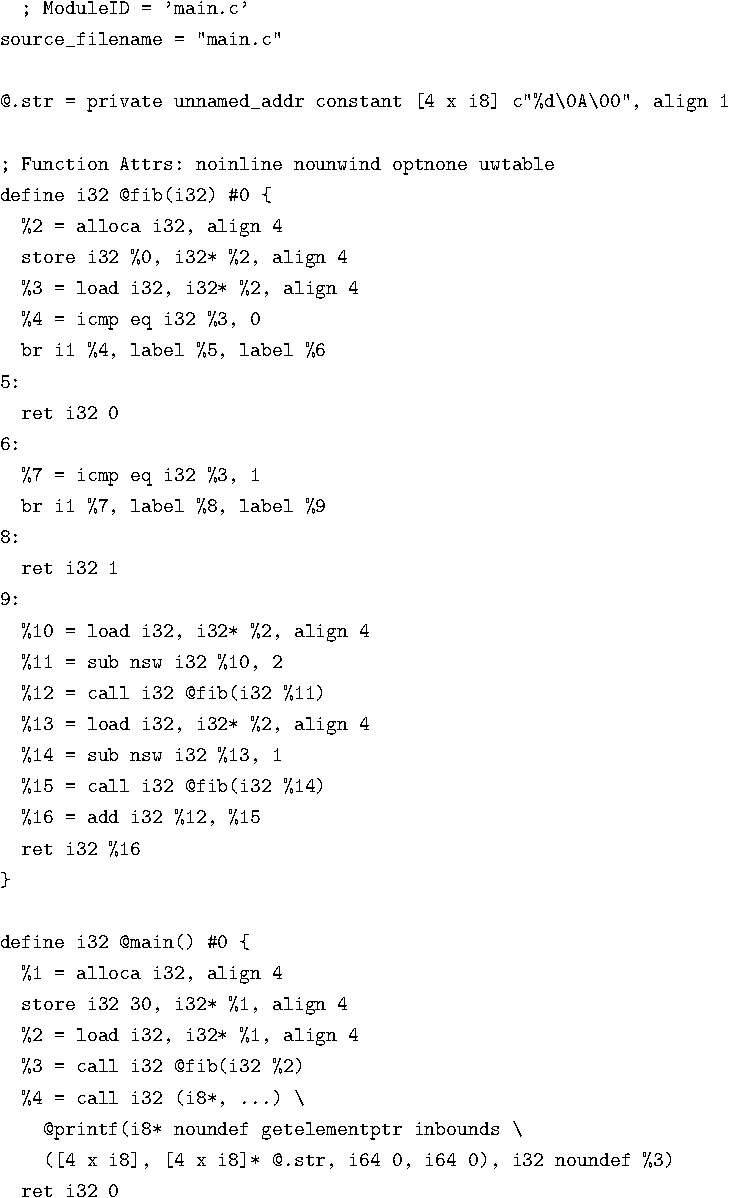
\includegraphics[scale=0.5]{fib_llvm-crop.pdf}
%   } & 
%   \multicolumn{1}{m{.5\textwidth}}{
%     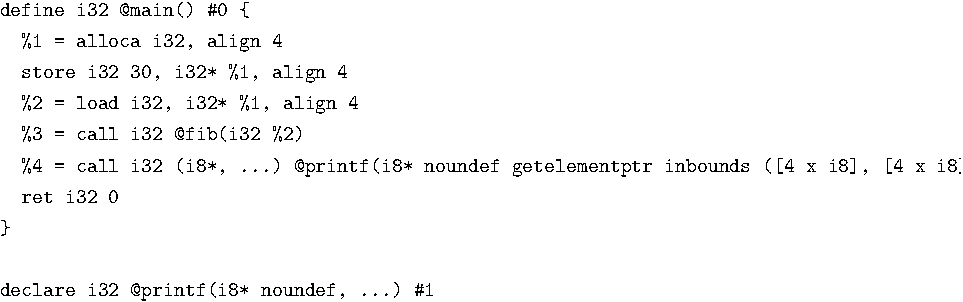
\includegraphics[scale=0.5]{fib_llvm2-crop.pdf}
%   }
% %  \begin{minipage}{.4\textwidth}
% % 
\includegraphics{Prog1_7_c.eps}
% % \vspace*{7cm}
% % \end{minipage}
% % &
% % 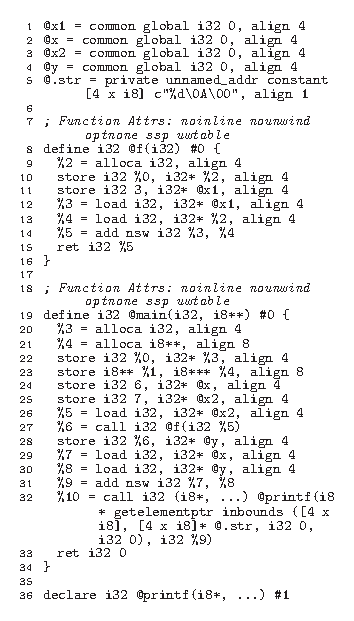
\includegraphics[height=.8\textheight]{Prog1_7_ll.eps}
% \end{tabularx}

% \end{frame}

\subsection{実行時環境}

\begin{frame}
  \frametitle{実行時環境}
  \greentext{メモリ領域の割り当て方}

  \begin{tabular}{ccc}
    \begin{minipage}{.5\textwidth}
      \begin{list}{$\bullet$}{}
        \item 大域変数=ヒープ領域(\greentext{プロセス内のメモリ領域})にわりあ
              てる。\\
              {\tt malloc},{\tt free}\\
              演習のコンパイラでは、スタック領域の底にわりあてる(popしない)。
        \item 局所変数=スタックにわりあてる
        \item 関数・手続の引数のわりあて(特殊な局所変数)
      \end{list}
    \end{minipage} & \quad &
    \begin{minipage}{.5\textwidth}
      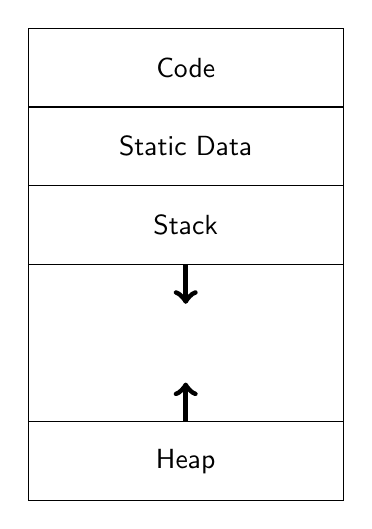
\begin{tikzpicture}
        \draw (0,0) rectangle (4,6);
        \node at (2,5.5) {Code};
        \draw (0,5) -- (4,5);
        \node at (2,4.5) {Static Data};
        \draw (0,4) -- (4,4);
        \node at (2,3.5) {Stack};
        \draw (0,3) -- (4,3);
        \draw (0,1) -- (4,1);
        \node at (2,0.5) {Heap};
        \draw [->,line width=2pt] (2,1) -- (2,1.5);
        \draw [->,line width=2pt] (2,3) -- (2,2.5);
      \end{tikzpicture}
    \end{minipage}
  \end{tabular}
\end{frame}

\begin{frame}
  \frametitle{静的割当てと動的割当て}
  \begin{tabular}{cc}
    \begin{minipage}{.5\textwidth}
      \begin{list}{}{}
        \item 静的割当て:
              \greentext{\small 実行の最初から最後までメモリ領域が変化しない}
        \item 動的割り当て：
              \greentext{\small メモリ領域が実行時に決定}\\
              \greentext{\small 実行終了時に領域が不要になる}
      \end{list}
    \end{minipage}
     &
    \begin{minipage}{.5\textwidth}
      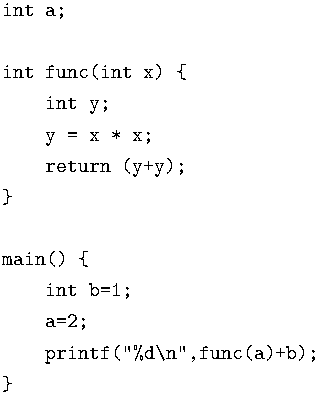
\includegraphics[scale=.75]{prog1.pdf}
    \end{minipage}
  \end{tabular}

  \begin{center}
    \begin{list}{}{}
      \item 静的割当て: {\tt a},{\tt func},{\tt main}
      \item 動的割当て: {\tt x},{\tt y},{\tt b}
    \end{list}
  \end{center}
\end{frame}

\subsection{駆動レコード}

\begin{frame}
  \frametitle{駆動レコード}
  手続き/関数の一回の実行に必要な局所情報\\
  \greentext{PC(Program Counter)、返り値、参照可能なシンボルの集合}

  \begin{center}
    \begin{tikzpicture}
      \draw[style=dotted] (3.5,2) -- (7.5,2);
      \draw[style=dotted] (3.5,1.5) -- (7.5,1.5);

      \draw (0,0) rectangle (1.5,1.5);
      \draw (0,0.5) -- (1.5,0.5);
      \draw (0,1) -- (1.5,1);
      \draw (1,1.5) -- (1,0);
      \node at (0.75,-.3) {実行前};
      \node at (0.5,0.25) {a};
      \node at (0.5,0.75) {func};
      \node at (0.5,1.25) {main};

      \draw (2,0) rectangle (3.5,2);
      \draw (2,0.5) -- (3.5,0.5);
      \draw (2,1) -- (3.5,1);
      \draw (2,1.5) -- (3.5,1.5);
      \draw (3,2) -- (3,0);
      \node at (2.75,-.3) {main実行中};

      \node at (2.5,0.25) {a};
      \node at (2.5,0.75) {func};
      \node at (2.5,1.25) {main};
      \node at (2.5,1.75) {b};

      \draw (4,0) rectangle (5.5,3);
      \draw (4,0.5) -- (5.5,0.5);
      \draw (4,1) -- (5.5,1);
      \draw (4,1.5) -- (5.5,1.5);
      \draw (4,2) -- (5.5,2);
      \draw (4,2.5) -- (5.5,2.5);
      \draw (5,0) -- (5,3);
      \node at (4.75,-.3) {func実行中};

      \node at (4.5,0.25) {a};
      \node at (4.5,0.75) {func};
      \node at (4.5,1.25) {main};
      \node at (4.5,1.75) {b};
      \node at (4.5,2.25) {x};
      \node at (4.5,2.75) {y};

      \node at (7,0.75) {大域変数};
      \node at (7.5,1.75) {mainのレコード};
      \node at (7.5,2.5) {funcのレコード};
    \end{tikzpicture}
  \end{center}

  % \begin{center}
  %  \includegraphics{activationRec1.eps}
  % \end{center}
\end{frame}

\begin{frame}
  \frametitle{駆動レコードの構成}

  \begin{tikzpicture}
    \draw (0,0) rectangle (4,4.8);
    \draw (0,0.6) -- (4,0.6);
    \draw (0,1.2) -- (4,1.2);
    \draw (0,1.8) -- (4,1.8);
    \draw (0,2.4) -- (4,2.4);
    \draw (0,3) -- (4,3);
    \draw (0,3.6) -- (4,3.6);
    \draw (0,4.2) -- (4,4.2);
    \node at (2,4.5) {一時変数領域};
    \node at (2,3.9) {局所データ領域};
    \node at (2,3.3) {静的リンク};
    \node at (2,2.7) {動的リンク};
    \node at (2,2.1) {戻り番地};
    \node at (2,1.5) {実引数計算領域};
    \node at (2,0.9) {戻り値};
    \node at (2,0.3) {退避領域};
    \draw[->] (4.5,2.7) -- (4,2.7);
    \node at (5,2.7) {FP};

    \node[anchor=west] at (5.5,4.5) {\greentext{関数内での計算の一時領域}};
    \node[anchor=west] at (5.5,3.9) {\greentext{局所宣言された変数の領域}};
    \node[anchor=west] at (5.5,3.3) {\greentext{次に外へ参照すべきレコード}};
    \node[anchor=west] at (5.5,2.7) {\greentext{Return後に復元すべきレコード}};
    \node[anchor=west] at (5.5,2.1) {\greentext{Return後に再開するPC}};
    \node[anchor=west] at (5.5,1.5) {\greentext{呼出の際に引数受け渡しに使う}};
    \node[anchor=west] at (5.5,0.9) {\greentext{関数の計算結果を格納}};
    \node[anchor=west] at (5.5,0.3) {\greentext{呼出の際の一時領域}};
  \end{tikzpicture}

  % \begin{pspicture}(0,0)(3,5)
  %  \psframe(0,0)(3,4)
  %  \rput(1.5,3.75){一時変数領域}
  %  \psline(0,3.5)(3,3.5)
  %  \rput(1.5,3.25){局所データ領域}
  %  \psline(0,3)(3,3)
  %  \rput(1.5,2.75){静的リンク}
  %  \psline(0,2.5)(3,2.5)
  %  \rput(1.5,2.25){動的リンク}
  %  \psline(0,2)(3,2)
  %  \rput(1.5,1.75){戻り番地}
  %  \psline(0,1.5)(3,1.5)
  %  \rput(1.5,1.25){実引数計算領域}
  %  \psline(0,1)(3,1)
  %  \rput(1.5,0.75){戻り値}
  %  \psline(0,0.5)(3,0.5)
  %  \rput(1.5,0.25){退避領域}
  %  \pnode(3,2.25){P1}
  %  \pnode(3.5,2.25){P2}
  %  \ncline{<-}{P1}{P2}
  %  \rput(4,2.25){FP}
  % \end{pspicture}
  % \begin{pspicture}(0,0)(4,5)
  %  \rput[l](1.25,3.75){\greentext{関数内での計算の一時領域(×)}}
  %  \rput[l](1.25,3.25){\greentext{局所宣言された変数の領域}}
  %  \rput[l](1.25,2.75){\greentext{\small スコープルールで次に外へ参照すべきレコード}}
  %  \rput[l](1.25,2.25){\greentext{Return後に復元すべきレコード}}
  %  \rput[l](1.25,1.75){\greentext{Return後に再開するPC}}
  %  \rput[l](1.25,1.25){\greentext{呼出の際に引数受け渡しに使う(×)}}
  %  \rput[l](1.25,0.75){\greentext{関数の計算結果を格納}}
  %  \rput[l](1.25,0.25){\greentext{呼出の際の一時領域(×)}}
  % \end{pspicture}

  % \vspace*{2em}
  %
  % (×)のところは演習では利用しない.
  % 動的リンクも不要
\end{frame}

% Insert demo

\newcommand{\commandPointer}[1]{\node[anchor=west,red] at ($#1*(0,0.5)+(-.45,0)$)  {$\rightarrow$};}

\begin{frame}[fragile]
  \frametitle{変数の参照}

  \begin{tikzpicture}
    \node[anchor=west] at (0,6.5)
    {\verb|int a;|};
    \node[anchor=west] at (0,6.0)
    {\verb|int func(int x) {|};
    \node[anchor=west] at (0,5.5)
    {\verb|  int y;|};
    \node[anchor=west] at (0,5.0)
    {\verb|  if(x==1) {return(a);}|};
    \node[anchor=west] at (0,4.5)
    {\verb|  else {|};
    \node[anchor=west] at (0,4.0)
    {\verb|    y=func(x-1)*2;|};
    \node[anchor=west] at (0,3.5)
    {\verb|    return(a+y);|};
    \node[anchor=west] at (0,3.0)
    {\verb|  }|};
    \node[anchor=west] at (0,2.5)
    {\verb|}|};
    \node[anchor=west] at (0,2.0)
    {\verb|void main() {|};
    \node[anchor=west] at (0,1.5)
    {\verb|  a=2;|};
    \node[anchor=west] at (0,1.0)
    {\verb|  printf("func(3)=%d",|};
    \node[anchor=west] at (0,0.5)
    {\verb|    func(3));|};
    \node[anchor=west] at (0,0)
    {\verb|}|};
    \draw (-0.5,-0.5) rectangle +(6.5,7.5);

    %    \only<2>{\node[anchor=west,red] at (-.45,1.5) {$\rightarrow$};}
    %    \only<3>{\node[anchor=west,red] at (-.45,1.0) {$\rightarrow$};}
    \only<2>{\commandPointer{3}}
    \only<3>{\commandPointer{2}}
    \only<4>{\commandPointer{10}}
    \only<5>{\commandPointer{8}}
    \only<6>{\commandPointer{10}}
    \only<7>{\commandPointer{8}}
    \only<8,9>{\commandPointer{10}}
    \only<10,11,12>{\commandPointer{8}}
    \only<13>{\commandPointer{7}}
    \only<14,15,16>{\commandPointer{8}}
    \only<17>{\commandPointer{7}}
    \only<18>{\commandPointer{3}}

    \only<1-16>{\node at (9,1.5) {\tt ?};}
    \only<1>{\node at (9,1) {\tt a=?};}
    \only<2->{\node at (9,1) {\tt a=2};}
    \only<4-17>{\node at (9,2) {\tt x=3};}
    \only<4-15>{\node at (9,2.5) {\tt y=?};}
    \only<4-17>{\draw (8,1.25) rectangle +(2,1.5);}
    \only<6-12>{\node at (9,3) {\tt ?};}
    \only<6-13>{\node at (9,3.5) {\tt x=2};}
    \only<6-11>{\node at (9,4) {\tt y=?};}
    \only<6-13>{\draw (8,2.75) rectangle +(2,1.5);}
    \only<8>{\node at (9,4.5) {\tt ?};}
    \only<8,9>{\node at (9,5) {\tt x=1};}
    \only<8,9>{\node at (9,5.5) {\tt y=?};}
    \only<8,9>{\draw (8,4.25) rectangle +(2,1.5);}
    \only<9,10>{\node at (9,4.5) {\tt 2};}
    \only<11>{\node at (9,4.5) {\tt 2*2};}
    \only<12,13>{\node at (9,4) {\tt y=4};}
    \only<13,14>{\node at (9,3) {\tt 6};}
    \only<15>{\node at (9,3) {\tt 6*2};}
    \only<16,17>{\node at (9,2.5) {\tt y=12};}
    \only<17,18>{\node at (9,1.5) {\tt 14};}

    \only<4-17>{\path[->,blue,line width=1.5pt] (8,2) edge [out=180,in=180] (8,1);}
    \only<6-13>{\path[->,blue,line width=1.5pt] (8,3.5) edge [out=180,in=180] (8,1);}
    \only<8,9>{\path[->,blue,line width=1.5pt] (8,5) edge [out=180,in=180] (8,1);}
    \only<4-17>{\node at (9,0) {\color{blue}静的リンク};}
  \end{tikzpicture}
\end{frame}

\begin{frame}
  \frametitle{変数の参照/記憶位置の決定}

  \begin{list}{}{}
    \item 局所変数: フレームポインタからの相対位置
    \item 大域変数: ヒープ内のアドレス\\
          %	(実習)：スタックボトムからの相対位置
  \end{list}

  % (実習)動的変数の位置：何番目に宣言されているか\\

  記号表にはスタックレームレジスタからの相対番地=何番目に宣言でどういった
  型をもつか。

  型情報=確保する領域量(実習の場は整数のみ)

  関数の引数うけわたしは局所変数の宣言+代入

\end{frame}

\section{構文主導型変換}

\subsection{意味解析}

\begin{frame}{動作意味}
  \[\langle\{S,E,T,F\},\{+,\ast,(,),n\},P,S
    \rangle\]
  \[\left\{\begin{array}{ll}
      S\rightarrow E\#,    & T\rightarrow F,       \\
      E\rightarrow E+T,    & F\rightarrow (\ E\ ), \\
      E\rightarrow T,      & F\rightarrow n,       \\
      T\rightarrow T\ast F &                       \\
    \end{array}\right\}\]

  \vspace*{3mm}

  \greentext{各生成規則は値を計算する意味を持つ．}

  \vspace*{3mm}

  $E\rightarrow E+T$: 右辺の$E$の値と$T$の値を加算した値を左辺の$E$の値とする．\\[3mm]
  $\Rightarrow$ \redtext{'+'に加算の意味を与える．}

\end{frame}

\begin{frame}{構文に従った動作意味}

  \[
    \begin{array}{ll}
      S\rightarrow E\#       & var(S)= var(E)               \\
      E\rightarrow E_1+T     & var(E)= var(E_1)+var(T)      \\
      E\rightarrow T         & var(E)=var(T)                \\
      T\rightarrow T_1\ast F & var(T)=var(T_1)\times var(F) \\
      T\rightarrow F         & var(T)=var(T)                \\
      F\rightarrow (\ E\ )   & var(F)=var(E)                \\
      F\rightarrow i         & temp=val(i);var(F)=temp
    \end{array}
  \]

  \vspace*{3mm}

  \greentext{構文主導型変換}

  \begin{description}
    \item [インタープリタ：] 生成規則に対応する動作をする．
    \item [コンパイラ：] 生成規則に対応した目的コード（中間コード）を生成する．
  \end{description}
\end{frame}

\subsection{中間コード生成ルーチン}


\begin{frame}
  \frametitle{構文主導型変換}
  CF文法の各生成規則に対してコード生成ルーチンをわりあてる。\\
  \begin{itemize}
    \item $\mathsf{newTemp}()$\\
          変数$T$の領域を確保して、記号番地または一時変数へのポインタを返す。
    \item $\mathsf{newLabel}()$\\
          新たなラベル名を返す。
    \item $\mathsf{generate}(\mbox{中間コード})$\\
          中間コードを出力ファイルに出力する。
  \end{itemize}

  \greentext{
    $n$回目に$\mathsf{newTemp}()$を呼びだしたとき、生成される
    変数$\texttt{t}n$}

  \greentext{
    $m$回目に$\mathsf{newLabel}()$を呼びだしたとき、生成されるラ
    ベル$\texttt{L}m$}

\end{frame}

\begin{frame}
  \frametitle{構文主導型変換の基礎}
  \begin{eqnarray*}
    S & \rightarrow & \mathsf{ID}\texttt{=}\ E\ \texttt{;}\\
    E & \rightarrow & E^{(1)}\ \texttt{+}\ \mathtt{NUM}\\
    E & \rightarrow & \mathtt{NUM}
  \end{eqnarray*}
  \begin{center}
    $\mathsf{ID}$\ $\texttt{=}$\ $\mathsf{NUM}_0$\ $\texttt{+}$\ $\mathsf{NUM}_1$
    \ $\texttt{+}$\ $\mathsf{NUM}_2$\ $\texttt{;}$
  \end{center}
  \begin{center}
    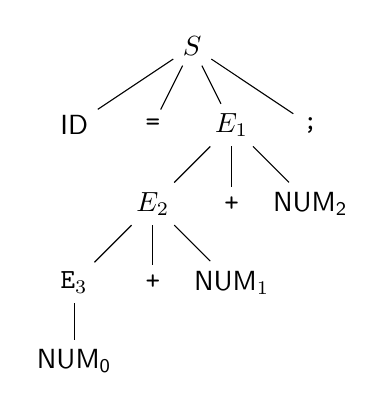
\begin{tikzpicture}
      \node (N0) at (0,0) {$\mathsf{NUM_0}$};
      \node (N1) at (0,1) {$\texttt{E}_3$};
      \node (N2) at (1,1) {$\texttt{+}$};
      \node (N3) at (2,1) {$\mathsf{NUM}_1$};
      \node (N4) at (1,2) {$E_2$};
      \node (N5) at (2,2) {$\texttt{+}$};
      \node (N6) at (3,2) {$\mathsf{NUM_2}$};
      \node (N7) at (0,3) {$\mathsf{ID}$};
      \node (N8) at (1,3) {$\texttt{=}$};
      \node (N9) at (2,3) {$E_1$};
      \node (N10) at (3,3) {$\texttt{;}$};
      \node (N11) at (1.5,4) {$S$};

      \path[-] (N0) edge (N1);
      \path[-] (N4) edge (N1) (N4) edge (N2) (N4) edge (N3);
      \path[-] (N9) edge (N4) (N9) edge (N5) (N9) edge (N6);
      \path[-] (N11) edge (N7) (N11) edge (N8) (N11) edge (N9) (N11) edge (N10);
    \end{tikzpicture}
    % \begin{pspicture}(0,0)(3,4)
    %  \rput(1.5,4){\rnode{P0}{$S$}}
    %  \rput(0,3){\rnode{P1}{$\mathsf{ID}$}}
    %  \rput(1,3){\rnode{P2}{$\mathtt{'='}$}}
    %  \rput(2,3){\rnode{P3}{$E_1$}}
    %  \rput(3,3){\rnode{P4}{$\mathtt{';'}$}}
    %  \rput(1,2){\rnode{P31}{$E_2$}}
    %  \rput(2,2){\rnode{P32}{$\mathtt{'+'}$}}
    %  \rput(3,2){\rnode{P33}{$\mathsf{NUM}_2$}}
    %  \rput(0,1){\rnode{P311}{$E_3$}}
    %  \rput(1,1){\rnode{P312}{$\mathtt{'+'}$}}
    %  \rput(2,1){\rnode{P313}{$\mathsf{NUM}_1$}}
    %  \rput(0,0){\rnode{P3111}{$\mathsf{NUM}_0$}}
    %  \ncline{-}{P0}{P1}
    %  \ncline{-}{P0}{P2}
    %  \ncline{-}{P0}{P3}
    %  \ncline{-}{P0}{P4}
    %  \ncline{-}{P3}{P31}
    %  \ncline{-}{P3}{P32}
    %  \ncline{-}{P3}{P33}
    %  \ncline{-}{P31}{P311}
    %  \ncline{-}{P31}{P312}
    %  \ncline{-}{P31}{P313}
    %  \ncline{-}{P311}{P3111}
    % \end{pspicture}

  \end{center}
\end{frame}

\begin{frame}
  \frametitle{中間コード(3番地コード)生成}
  \begin{center}
    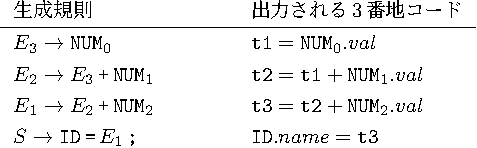
\includegraphics[scale=.8]{prodcode1-crop.pdf}
  \end{center}
  \begin{center}
    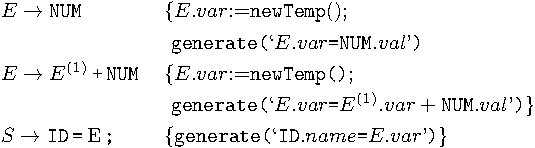
\includegraphics[scale=.8]{code-prog-r1-crop.pdf}
  \end{center}
\end{frame}
\begin{frame}
  \frametitle{IF文の中間コード生成}
  \only<1>{
    \[
      \mbox{文}\ \rightarrow\ \mathsf{if}\ \mathtt{'('}\ \mbox{式}\
      \mathtt{')'}\ \mbox{文}^{(1)}
    \]
    \begin{enumerate}
      \item '式'のコードを生成 {\sf t1}に結果収納
      \item {\sf if not t1 goto l1}
      \item '文'$^{(1)}$のコードを生成
      \item {\sf l1:}
    \end{enumerate}
  }
  \only<2>{
    \[
      \mbox{文}\ \rightarrow\ \mathsf{if}\ \mathtt{'('}\ \mbox{式}\
      \mathtt{')'}\ \mbox{文}^{(1)}\ \mathsf{else}\ \mbox{文}^{(2)}
    \]
    \begin{enumerate}
      \item '式'のコードを生成 {\sf t1}に結果収納
      \item {\sf if not t1 goto l1}
      \item '文'$^{(1)}$のコードを生成
      \item {\sf goto l2}
      \item {\sf l1:}
      \item '文'$^{(2)}$のコードを生成
      \item {\sf l2:}
    \end{enumerate}
  }
\end{frame}
\begin{frame}
  \frametitle{while文の中間コード生成}
  \[
    \mbox{文}\ \rightarrow\ \mathsf{while}\ \mathtt{'('}\ \mbox{式}\
    \mathtt{')'}\ \mbox{文}^{(1)}
  \]
  \begin{enumerate}
    \item {\sf l1:}
    \item '式'のコードを生成 {\sf t1}に結果収納
    \item {\sf if not t1 goto l2}
    \item '文'$^{(1)}$のコードを生成
    \item {\sf goto l1}
    \item {\sf l2:}
  \end{enumerate}
\end{frame}


\begin{frame}
  \frametitle{構文主導型変換によるコード生成}
  {\small
    \begin{tabular}{lll}
      文$\rightarrow$ & {\tt if} (  & \{文.label:=\makenewlabel;\}                                \\
                     & 式           & (式のコード)                                                    \\
                     & )           & \{\genifnot{式.var}{文.label}\}                              \\
                     & 文$^{(1)}$   & (文$^{(1)}$のコード)\{\genlabel{文.label};                       \\
                     &             & 文$^{(1)}$.label:=\makenewlabel;\gengoto{文$^{(1)}$.label}\} \\
                     & {\tt else}  & \{\genlabel{文.label}\}                                     \\
                     & 文{$^{(2)}$} & \{\genlabel{文$^{(1)}$.label}\}
    \end{tabular}

    \vspace*{1zw}

    \begin{tabular}{lll}
      文$\rightarrow$ & {\tt while} ( & \{文.label1:=\makenewlabel;   \\
                     &               & \genlabel{文.label1}\}        \\
                     & 式             & (式のコード)                      \\
                     & )             & \{文.label2:=\makenewlabel;   \\
                     &               & \genifnot{式.var}{文.label2}\} \\
                     & 文$^{(1)}$     & (文のコード)                      \\
                     &               & \{\gengoto{文.label1};        \\
                     &               & \genlabel{文.label2}\}        \\
    \end{tabular}
  }
\end{frame}

\subsection{中間コード生成ルーチン}

\begin{frame}
  \frametitle{PDTを用いた構文主導型変換}
  \greentext{コード生成を行うタイミング=還元操作}
  \begin{center}
    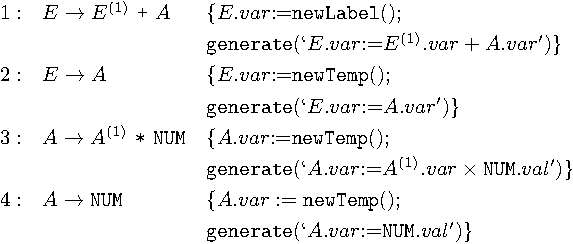
\includegraphics[scale=0.6]{bup-SDD-r1-crop.pdf}
  \end{center}
  \begin{center}
    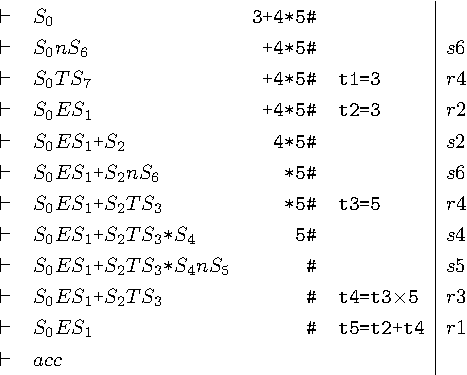
\includegraphics[scale=0.5]{IR-gen-crop.pdf}
  \end{center}
\end{frame}

\begin{frame}
  \frametitle{変換例}
  \[
    \begin{array}{ll}
      E_1\rightarrow a\ast b       & \{\%0=a\ast b\}  \\
      E_2\rightarrow -d            & \{\%1=-d\}       \\
      E_3\rightarrow c\ast E_2     & \{\%2=c\ast\%1\} \\
      E_4\rightarrow E_1+E_2       & \{\%3=\%0+\$2\}  \\
      S\rightarrow x\texttt{:=}E_3 & \{x=\%3\}
    \end{array}
  \]

  \begin{tikzpicture}
    \node (X0) at (0,0) {$x$};
    \node (T1) at (0.75,0) {$:=$};
    \node (T2) at (1.5,0) {$a$};
    \node (T3) at (2,0) {$\ast$};
    \node (T4) at (2.5,0) {$b$};
    \node (T5) at (3,0) {$+$};
    \node (T6) at (3.5,0) {$c$};
    \node (T7) at (4,0) {$\ast$};
    \node (T8) at (4.5,0) {$-$};
    \node (T9) at (5,0) {$d$};
    \uncover<2->{\node (T10) at (2,1) {$E_1$};}
    \uncover<3->{\node (T11) at (4.75,1) {$E_2$};}
    \uncover<4->{\node (T12) at (3.5,2) {$E_3$};}
    \uncover<5->{\node (T13) at (3,3) {$E_4$};}
    \uncover<6->{\node (T14) at (2,4) {$S$};}

    \uncover<2->{\path[-] (T2) edge (T10) (T3) edge (T10) (T4) edge (T10);}
    \uncover<3->{\path[-] (T8) edge (T11) (T9) edge (T11);}
    \uncover<4->{\path[-] (T6) edge (T12) (T7) edge (T12) (T11) edge (T12);}
    \uncover<5->{\path[-] (T10) edge (T13) (T5) edge (T13) (T12) edge (T13);}
    \uncover<6->{\path[-] (X0) edge (T14) (T1) edge (T14) (T13) edge (T14);}

    \only<2->{\node (N10) at (2.5,1) {\redtext{$\%0$}};}
    \only<3->{\node (N11) at (5.25,1) {\redtext{$\%1$}};}
    \only<4->{\node (N12) at (4,2) {\redtext{$\%2$}};}
    \only<5->{\node (N13) at (3.5,3) {\redtext{$\%3$}};}
    \only<6->{\node (N14) at (2.5,4) {\redtext{$\%4$}};}

    \only<2->{\node[anchor=west] at (6,3.5) {$\%0=a\ast b$};}
    \only<3->{\node[anchor=west] at (6,3) {$\%1=-d$};}
    \only<4->{\node[anchor=west] at (6,2.5) {$\%2=c\ast\% 1$};}
    \only<5->{\node[anchor=west] at (6,2) {$\%3=\$ 0+\% 2$};}
    \only<6->{\node[anchor=west] at (6,1.5) {$x=\%3$};}
  \end{tikzpicture}
\end{frame}

\begin{frame}
  \frametitle{条件分岐に対する構文主導型変換}

  %\greentext{LR項の状態に対してコード生成}

  \greentext{分岐条件の評価の後に分岐命令を生成する必要がある．}

  \vfill

  \begin{tabular}{cc}
    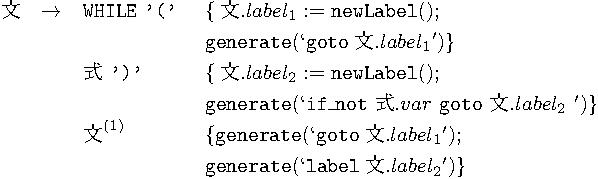
\includegraphics[width=.7\textwidth]{whileTrans-r1-crop.pdf} &
    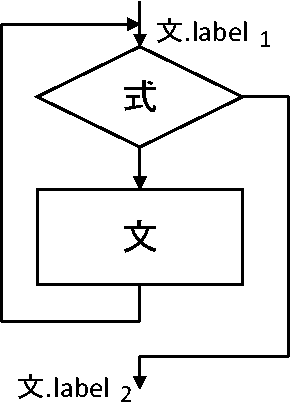
\includegraphics[width=.2\textwidth]{whileFlow-crop.pdf}
  \end{tabular}

  %  \begin{trivlist}
  %   \item  $\mathsf{newLabel}(\&\mbox{文}.label_1)$:\\
  % 	 新たなラベルを生成して,$\mbox{文}.label_1$の値を更新する.
  %   \item $\mathsf{generate}(s1,s2,\ldots)$:\\
  % 	$s_1,s_2,\ldots$ の命令部分を結合して命令を生成する.
  %   \item $\mbox{式}.var$:\\
  % 	式のコード生成の結果が格納される変数
  %  \end{trivlist}

\end{frame}

\begin{frame}[fragile]
  \frametitle{while文の中間コード生成例}
  \begin{center}
    \begin{Verbatim}
      while(x<20) {
          r=r+x;
          x=x+1
        }
    \end{Verbatim}
  \end{center}
  \begin{tabular}{cc}
    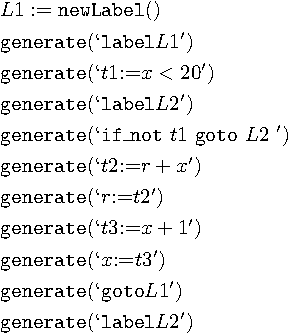
\includegraphics[width=.3\textwidth]{whileCodeExample-r1-crop.pdf}
     &
    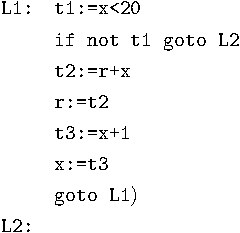
\includegraphics[width=.3\textwidth]{whileCode-crop.pdf}
    \\
  \end{tabular}
\end{frame}

\begin{frame}
  \frametitle{上昇型構文解析におけるコード生成}

  \begin{trivlist}
    \item IF文
    {\small
    \[\begin{array}{rcll}
        I  & \rightarrow                       & \texttt{if}\ \texttt{(}\ E\ \texttt{)}
           & \{S.label1\mbox{:=\makenewlabel};                                                                         \\
           &                                   &                                        & \genifnot{E.var}{S.label1}\} \\
        S' & \rightarrow\                      & I S^{(1)}                              & \{S'.label:=\makenewlabel;   \\
           &                                   &                                        & \gengoto{S'.label};          \\
           &                                   &                                        & \genlabel{I.label}\}         \\
        S  & \rightarrow                       & S'\ \texttt{else}\ S^{(2)}             & \{\genlabel{S'.label}\}      \\
      \end{array}\]}
    \item WHILE文
    {\small
    \[\begin{array}{rcll}
        I  & \rightarrow & \texttt{while}\ \texttt{(} & \{I.label\mbox{:=}\makenewlabel; \\
           &             &                            & \genlabel{I.label}\}             \\
        S' & \rightarrow & E\ \texttt{)}              & \{S'.label:=\makenewlabel;       \\
           &             &                            & \genifnot{E.var}{S'.label}\}     \\
        S  & \rightarrow & IS'S^{(1)}                 & \{\gengoto{I.label};             \\
           &             &                            & \genlabel{S'.label}\}
      \end{array}\]}
  \end{trivlist}
\end{frame}

\begin{frame}
  \frametitle{下降型構文主導型変換}
  構文図式に従ってコードを生成する。

  \greentext{丸}の部分でコードを生成する

  \begin{center}
    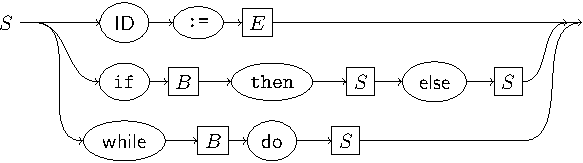
\includegraphics[scale=.8]{synDiag-S-crop.pdf}
  \end{center}
\end{frame}

\begin{frame}
  \begin{center}
    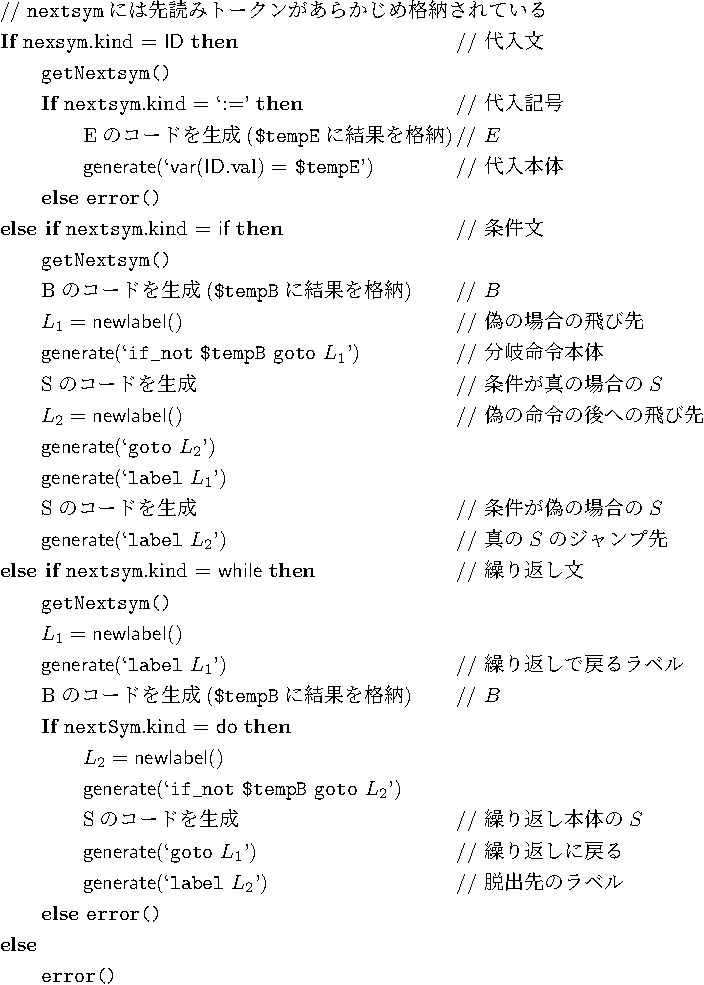
\includegraphics[scale=.5]{recDescent-gen-crop.pdf}
  \end{center}
\end{frame}

\begin{frame}
  \frametitle{属性文法}

  属性文法(attribute grammar):抽象構文木に属性を加えた文法

  \greentext{構文主導型変換への応用=コード生成に関する情報を属
    性として扱う}

  属性文法 $A_g=(G,{\cal A},E)$
  \begin{list}{}{}
    \item $G=(N,\Sigma,P,S)$はCF文法
    \item ${\cal A}$:属性の集合\\
          ${\cal A}=\cup_{X\in
              N\cup\Sigma}{\cal A}(X)$.  $a\in{\cal A}(X)$のとき、
          $X.a$と書く。
    \item $E$:意味規則の集合\\
          $p\in P$に対して以下のような規則定める。
          \[
            p\{X_i.a_i=f_i(X_{i_1}.a_{i_1},\ldots,X_{i_n}.a_{i_n})\}
          \]
  \end{list}

  \[\begin{array}{ll}
      E\rightarrow E^{(1)}\texttt{+}E^{(2)} & \{E.val=E^{(1)}.val+E^{(2)}.val\} \\
      E\rightarrow \texttt{NUM}             & \{E.val=\texttt{NUM}.val\}
    \end{array}
  \]
  %  \begin{center}
  %   \includegraphics[scale=1]{figs191113/attribGram01.eps}
  %  \end{center}

\end{frame}


\begin{frame}
  \frametitle{属性の種類}

  \begin{list}{}{}
    \item 合成(synthesized)属性\\
          \greentext{右辺の属性から合成された左辺の属性}:
    \item 相続(inherited)属性 (「継承属性」とも言う)\\
          \greentext{合成以外の属性}
  \end{list}


  \[G=(\{T,L\},\{\texttt{MAX},\texttt{MIN},\texttt{NUM},`\texttt{(}',`\texttt{)}',`\texttt{,}'\},P,T)\]

  \scalebox{0.8}{
    $\mathcal{A}$:
    \begin{tabular}{|c|c|c|}\hline
          & 合成属性    & 相続属性   \\\hline
      $T$ & $T.val$ &        \\\hline
      $L$ & $L.val$ & $L.op$ \\\hline
    \end{tabular}
  }

  \vspace*{5pt}

  {\small
    %P,E:\\

    $P=\left\{\begin{array}{ll}
        T\rightarrow\texttt{MIN'('}L\texttt{')'} & \{L.op=\texttt{MIN},T.val=L.val\}                                  \\
        T\rightarrow\texttt{MAX'('}L\texttt{')'} & \{L.op=\texttt{MAX},T.val=L.val\}                                  \\
        L\rightarrow\texttt{NUM}                 & \{L.val=\texttt{NUM}.val\}                                         \\
        L\rightarrow L^{(1)}\texttt{',' NUM}     & \left\{\begin{array}{l}L.val=f(L.op,L^{(1)}.val,\texttt{NUM}.val), \\
                                                            L^{(1)}.op=L.op\end{array}\right\}
      \end{array}\right\}$
  }
  %  \begin{center}
  %   \includegraphics[scale=.8]{figs191113/AttributeExample.eps}
  %  \end{center}
\end{frame}

\begin{frame}
  \frametitle{属性文法に基づくコード生成例}
  $G$に生成規則$\{S\rightarrow T\#\}$を加えた拡張文法に対するLR解析

  \vspace*{3pt}

  $P=\left\{\begin{array}{rlcrl}
      0: & S\rightarrow T\#,                                        &  & 3: & L\rightarrow\texttt{NUM},                   \\
      1: & T\rightarrow\texttt{MIN}\ `\texttt{(}'\ L\ `\texttt{)}', &  & 4: & L\rightarrow L\ `\texttt{,}'\ \texttt{NUM}, \\
      2: & T\rightarrow\texttt{MAX}\ `\texttt{(}'\ L\ `\texttt{)}'  &  &    &
    \end{array}\right\}$

  \vspace*{3pt}

  $\mathsf{Follow}_1(T)=\{\#\}$,
  $\mathsf{Follow}_1(L)=\{\texttt{)},`\texttt{,}'\}$


\end{frame}

\begin{frame}
  \frametitle{属性文法に基づくコード生成例}
  \begin{center}
    \begin{tabularx}{\textwidth}{XX}
      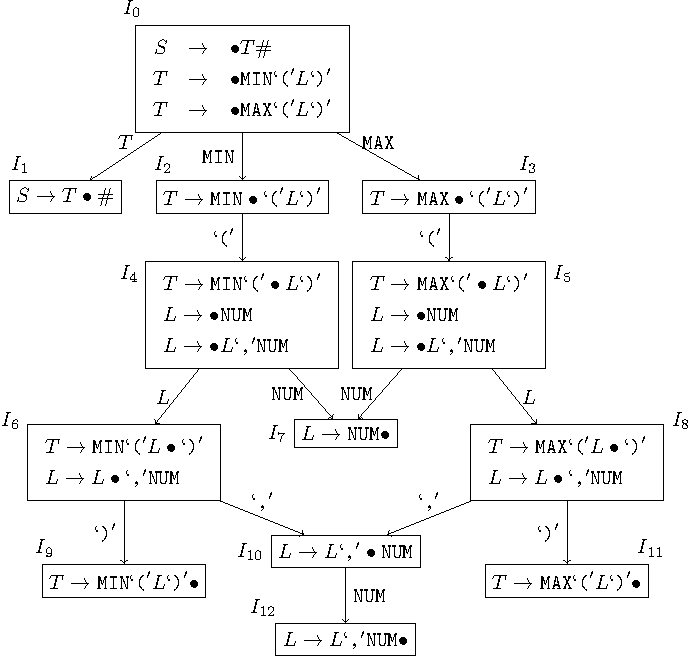
\includegraphics[scale=0.45]{maxmin-lrautomaton-crop.pdf}
                        &
      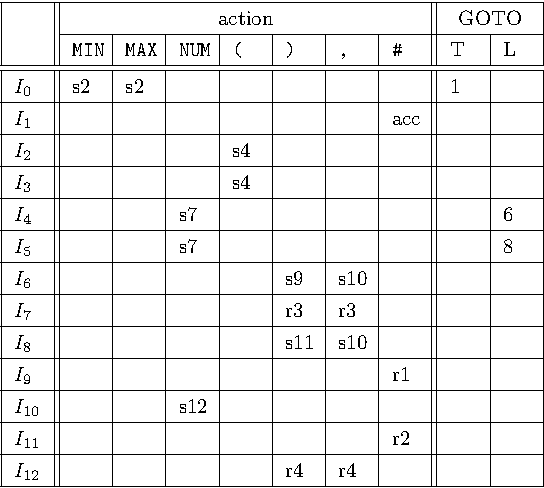
\includegraphics[scale=0.5]{maxmin-parsetab-crop.pdf} \\
      {\small LR(0)遷移系} & {\small SLR(1)構文解析表}
    \end{tabularx}
  \end{center}
\end{frame}

\begin{frame}
  \frametitle{属性文法に基づくコード生成例}
  \scriptsize{
    \[
      \begin{array}{clllll}
                  & (I_0,                                                          & \texttt{MIN(3,5,7)\#}, & \varepsilon)                                                                 \\
        \vdash    & (I_0\texttt{MIN}I_2,                                           & \texttt{(3,5,7)\#},    & \varepsilon)                                                                 \\
        \vdash    & (I_0\texttt{MIN}I_2\texttt{(}I_4,                              & \texttt{3,5,7)\#},     & \varepsilon)                                                                 \\
        \vdash    & (I_0\texttt{MIN}I_2\texttt{(}I_4\texttt{3}I_7,                 & \texttt{,5,7)\#},      & \varepsilon)                                                                 \\
        \vdash    & (I_0\texttt{MIN}I_2\texttt{(}I_4 L I_6,                        & \texttt{,5,7)\#},      & 3)           & \%1.val=3                                                     \\
        \vdash    & (I_0\texttt{MIN}I_2\texttt{(}I_4 L I_6\texttt{,}I_{10},        & \texttt{5,7)\#},       & 3)                                                                           \\
        \vdash    & (I_0\texttt{MIN}I_2\texttt{(}I_4 L I_6\texttt{,}I_{10}5I_{12}, & \texttt{,7)\#},        & 3)                                                                           \\
        \vdash    & (I_0\texttt{MIN}I_2\texttt{(}I_4 L I_6,                        & \texttt{,7)\#},        & 34)          & \%2.val=f(\only<1>{\%1.op}\only<2>{\redtext{min}},\%1.val,5); \\
        \only<1>{ &                                                                &                        &              & \%2.op=\%1.op\\}
        \vdash    & (I_0\texttt{MIN}I_2\texttt{(}I_4 L I_6\texttt{,}I_{10},        & \texttt{7)\#},         & 34)                                                                          \\
        \vdash    & (I_0\texttt{MIN}I_2\texttt{(}I_4 L I_6\texttt{,}I_{10}7I_{12}, & \texttt{)\#},          & 34)                                                                          \\
        \vdash    & (I_0\texttt{MIN}I_2\texttt{(}I_4 L I_6,                        & \texttt{)\#},          & 344)         & \%3.val=f(\only<1>{\%2.op}\only<2>{\redtext{min}},\%2.val,7); \\
        \only<1>{ &                                                                &                        &              & \%3.op=\%2.op\\}
        \vdash    & (I_0\texttt{MIN}I_2\texttt{(}I_4 L I_6\texttt{)}I_9,           & \texttt{\#},           & 344)                                                                         \\
        \vdash    & (I_0 T I_1,                                                    & \texttt{\#},           & 3441)        & \only<1>{\redtext{\%3.op=min;}}\%4.val=\%3.val                \\
        \vdash    & (acc,                                                          & \texttt{\#},           & 34410)
      \end{array}
    \]
  }
  \only<1>{\greentext{相続属性($f$の第一引数)が最後に決定される}}
  \only<2>{\greentext{相続属性($f$の第一引数)をバックパッチによって関数を書き換える}}

  $T.val=\%4.val$
\end{frame}

\begin{frame}
  \frametitle{属性文法に基づくコード生成例}
  \scriptsize{
    \[
      \begin{array}{clllll}
                  & (I_0,                                                          & \texttt{MAX(3,5,7)\#}, & \varepsilon)                                                                   \\
        \vdash    & (I_0\texttt{MAX}I_2,                                           & \texttt{(3,5,7)\#},    & \varepsilon)                                                                   \\
        \vdash    & (I_0\texttt{MAX}I_2\texttt{(}I_4,                              & \texttt{3,5,7)\#},     & \varepsilon)                                                                   \\
        \vdash    & (I_0\texttt{MAX}I_2\texttt{(}I_4\texttt{3}I_7,                 & \texttt{,5,7)\#},      & \varepsilon)                                                                   \\
        \vdash    & (I_0\texttt{MAX}I_2\texttt{(}I_4 L I_6,                        & \texttt{,5,7)\#},      & 3)           & \%1.val=3                                                       \\
        \vdash    & (I_0\texttt{MAX}I_2\texttt{(}I_4 L I_6\texttt{,}I_{10},        & \texttt{5,7)\#},       & 3)                                                                             \\
        \vdash    & (I_0\texttt{MAX}I_2\texttt{(}I_4 L I_6\texttt{,}I_{10}5I_{12}, & \texttt{,7)\#},        & 3)                                                                             \\
        \vdash    & (I_0\texttt{MAX}I_2\texttt{(}I_4 L I_6,                        & \texttt{,7)\#},        & 34)          & \%2.val=f(\only<1>{\%1.op}\only<2>{\greentext{max}},\%1.val,5); \\
        \only<1>{ &                                                                &                        &              & \%1.op=\%2.op\\}
        \vdash    & (I_0\texttt{MAX}I_2\texttt{(}I_4 L I_6\texttt{,}I_{10},        & \texttt{7)\#},         & 34)                                                                            \\
        \vdash    & (I_0\texttt{MAX}I_2\texttt{(}I_4 L I_6\texttt{,}I_{10}7I_{12}, & \texttt{)\#},          & 34)                                                                            \\
        \vdash    & (I_0\texttt{MAX}I_2\texttt{(}I_4 L I_6,                        & \texttt{)\#},          & 344)         & \%3.val=f(\only<1>{\%2.op}\only<2>{\greentext{max}},\%2.val,7); \\
        \only<1>{ &                                                                &                        &              & \%2.op=\%3.op\\}
        \vdash    & (I_0\texttt{MAX}I_2\texttt{(}I_4 L I_6\texttt{)}I_9,           & \texttt{\#},           & 344)                                                                           \\
        \vdash    & (I_0 T I_1,                                                    & \texttt{\#},           & 3442)        & \only<1>{\redtext{\%3.op=max;}}\%4.val=\%3.val                  \\
        \vdash    & (acc,                                                          & \texttt{\#},           & 34410)
      \end{array}
    \]
  }

  \only<1>{\greentext{相続属性($f$の第一引数)が最後に決定される}}
  \only<2>{\greentext{相続属性($f$の第一引数)をバックパッチによって関数を書き換える}}

  $T.val=\%4.val$

\end{frame}

% \subsection{バックパッチ}

% \begin{frame}
%  \frametitle{バックパッチ}

%  条件分岐のコード生成の場合、ラベルの値はあとで決定する

%  \[
% p  \mathsf{if}\ E\ \mathsf{then}\ S
%  \]

% \begin{center}
%  \begin{tabular}{lrl}
% 1:&    & $E$のコード\\
% 2:&    & if not $E.\mathsf{result}$ goto $L$\\
% 3:&    & $S$のコード\\
% 4:&$L$:&
%  \end{tabular}
% \end{center}

%  $S$をコンパイルするまで$L$の値は決まらない。2の時点で$L$の具
%  体的なアドレスはわからない。

% % 厳密には1パスでコード生成はできない。

% \begin{list}%
%  {$\bullet$} %default label
%  {} %formatting parameter
%  \item とび先のアドレスの表を作成しておいて、アドレスが決定した時点で
%  $L$の値を待つコードをかきかえる。 
%  \item 命令を一旦生成するがどこが未決かを管理する。
% \end{list}

% \greentext{LLVM 実行系においては，LLVM抽象マシンがラベルを解決してくれる．}

% \end{frame}



\begin{frame}{LLVMによる条件文コード}

  \texttt{if} {$B$} \texttt{then} {$S_1$} \texttt{else} {$S_2$}

  \vspace*{5mm}

  \begin{tabular}{l}
    \texttt{\%1 = } [$B$ を計算するコード]             \\
    \texttt{br i1 \%1, label \%L1, label \%L2} \\
    \texttt{L1:}                               \\
    \quad [$S_1$のコード]                          \\
    \texttt{br label \%L3}                     \\
    \texttt{L2:}                               \\
    \quad [$S_2$のコード]                          \\
    \texttt{br label \%L3}                     \\
    \texttt{L3:}
  \end{tabular}

  \greentext{\texttt{L1},\texttt{L2},\texttt{L3}は実際に定義される前に参照される．}

  \greentext{$S_2$の後の\%3へのジャンプは不要．}

\end{frame}

\begin{frame}[fragile]
  \frametitle{条件文における論理式}
  条件文における条件の評価：結果待ち / 短絡型\\
  \greentext{条件が副作用を持つ場合に違いが出る}\\
  \texttt{if (x>100 \&\& (z=y)<30) \{ 文1 \} else \{ 文2 \}}\\
  \texttt{z=y}の評価結果は\texttt{y}の値\\
  \greentext{{\tt z=y}が実行されるか？}\\
  結果待ち=評価される、短絡型=\texttt{x>100}のとき評価される\\

  \begin{tabular}{ll}
    短絡型： & 条件文の評価中にif文を評価する．    \\
    結果待： & 条件文の式を評価してからifを評価する．
  \end{tabular}

  \greentext{短絡型の評価を行う場合が多い(C, python)}

  \greentext{javaの場合：\texttt{\&\&},\texttt{||}が短絡型，\texttt{\&},\texttt{|}が結果待ち}
  %\greentext{java: $\texttt{\&\&}$, $\texttt{\|\|}$は短絡型，\texttt{\&}, \texttt{|}は結果待ち}

  %  \begin{verbatim}
  %    t1:=x>100;if not t1 goto L1;
  %    t2:=y;z:=t2;t4:=t2<30;if not t4 goto L1;
  %    文1.code; goto L2;
  % L1:文2.code;
  % L2:
  %  \end{verbatim}
  %  \greentext{文1を読まないと、L1が決定しない。}\\
  %  \greentext{文2を読まないと、L2が決定しない。}
\end{frame}

\section{関数}

\subsection{引数受け渡し}

\begin{frame}
  \frametitle{関数引数・返り値と駆動レコード}

  \begin{tabular}{ccc}
    \begin{minipage}{.4\textwidth}
      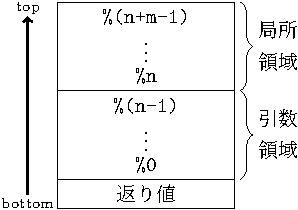
\includegraphics{activeRecord-crop.pdf}
    \end{minipage}
     & \quad &
    \begin{minipage}{.45\textwidth}
      $\texttt{f}(x_1,\cdots,x_n)$でスタック上に
      作成される駆動レコード（の一部）\\
      局所変数: $y_1,\cdots,y_m$\\[10pt]
      \greentext{これに従った記号表を生成}
    \end{minipage}
  \end{tabular}

  \vspace*{10pt}

  \begin{description}
    \item [値呼び：]
          $\texttt{x=f(}e_1,\cdots,e_n\texttt{)}$\\
          $e_i$を評価してその値を$x_i$の領域にコピー
    \item [参照呼び：]
          $\texttt{x=f(}z_1,\cdots,z_n\texttt{)}$\\
          $z_i$のアドレスを$x_i$にコピー
  \end{description}
\end{frame}

\begin{frame}[fragile=singleslide]
  \frametitle{引数受渡し}
  \greentext{引数=パラメータ(parameter)}\\
  2種類の受渡し方法
  \begin{list}{}{}
    \item 値渡し：実引数の値を評価して仮引数に代入
    \item 参照渡し：実引数の値を評価して\underline{ポインタ}を仮引数に代入
  \end{list}

  \vfill

  \begin{center}
    \begin{tabular}{ccc}
      \multicolumn{1}{c}{値呼び} & \multicolumn{1}{c}{} & \multicolumn{1}{c}{参照呼び} \\\cline{1-1}\cline{3-3}
      \multicolumn{1}{|m{.35\textwidth}|}{
      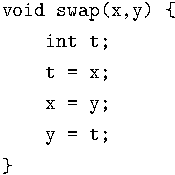
\includegraphics[scale=.8]{swap-value-crop.pdf}
      }
                              &                      &
      \multicolumn{1}{|m{.4\textwidth}|}{
      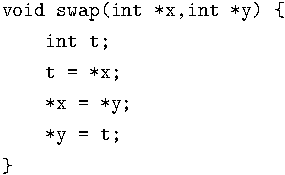
\includegraphics[scale=.8]{swap-ref-crop.pdf}}
      \\\cline{1-1}\cline{3-3}
    \end{tabular}
  \end{center}

  \begin{list}{}{}
    \item 値呼びの場合：全く効果なし。\\
          \greentext{入れ替えられた値は駆動レコード内で実行後破棄}
    \item 参照呼びの場合：値が入れ替えられる。\\
          \greentext{{\tt swap}中の{\tt y=x}, {\tt x=t}の代入先は、
          実引数の領域}
  \end{list}
\end{frame}

\begin{frame}
  \frametitle{値呼びのコンパイル}
  \%0: xの値，\%1: yの値が格納されているアドレス

  \vspace*{5pt}

  \begin{center}
    \begin{tabular}{cc}
      \multicolumn{1}{m{.3\textwidth}}{
        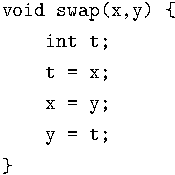
\includegraphics[scale=.8]{swap-value-crop.pdf}}
       &
      \multicolumn{1}{m{.5\textwidth}}{
        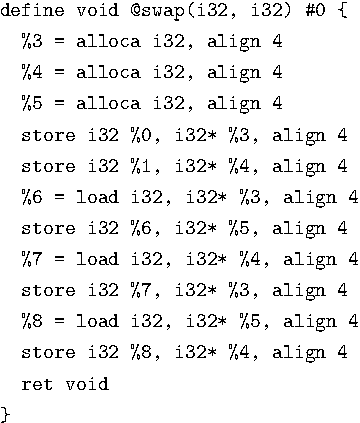
\includegraphics[scale=.7]{swap-v-ll-crop.pdf}}
    \end{tabular}
  \end{center}
\end{frame}

\begin{frame}
  \frametitle{参照呼びのコンパイル}
  \%0: xの値，\%1: yの値が格納されているアドレス

  \vspace*{5pt}

  \begin{center}
    \begin{tabular}{cc}
      \multicolumn{1}{m{.4\textwidth}}{
        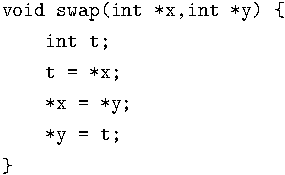
\includegraphics[scale=.8]{swap-ref-crop.pdf}}
       &
      \multicolumn{1}{m{.5\textwidth}}{
        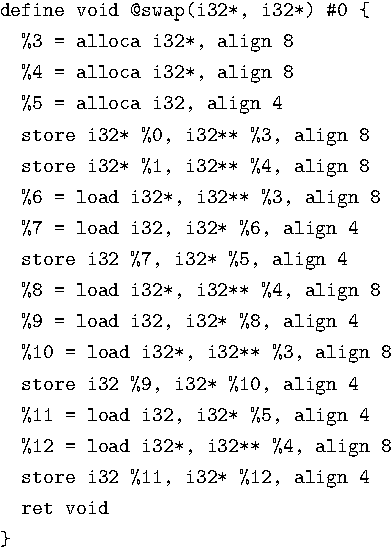
\includegraphics[scale=.7]{swap-ref-ll-crop.pdf}}
    \end{tabular}
  \end{center}
\end{frame}

\subsection{関数定義}

\begin{frame}[fragile]{関数定義/値呼び}

  \scalebox{0.75}{
    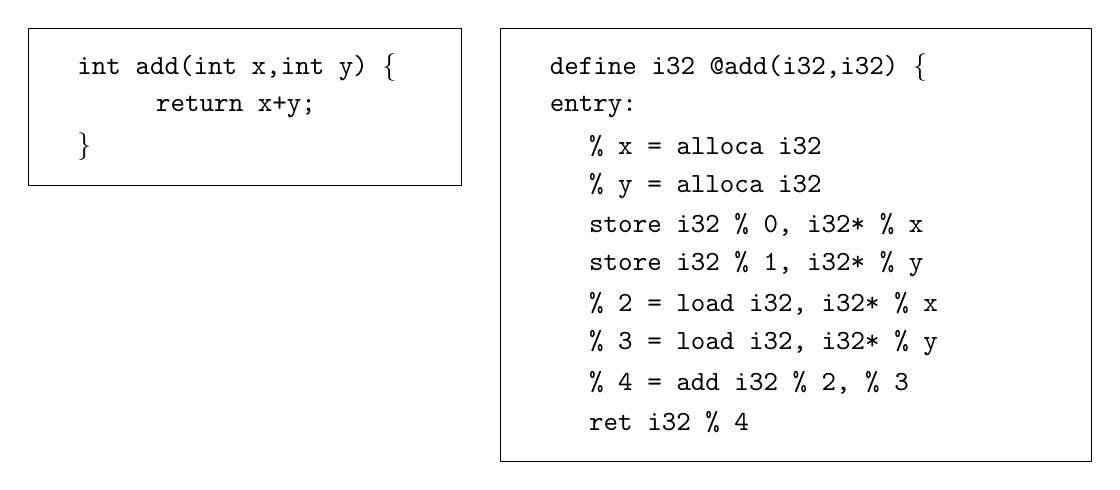
\begin{tikzpicture}
      \draw[draw] (-0.5,0.5) rectangle (5,-1.5);
      \node[anchor=west] (L01) at (0,0) {\texttt{int add(int x,int y) \{}};
      \node[anchor=west] at (1,-0.5) {\texttt{return x+y;}};
      \node[anchor=west] at (0,-1) {\texttt{\}}};

      \draw[draw] (5.5,0.5) rectangle (13,-5);
      \node[anchor=west] at (6,0) {\texttt{define i32 @add(i32,i32) \{}};
      \node[anchor=west] at (6,-0.5) {\texttt{entry:}};
      \node[anchor=west] at (6.5,-1) {\texttt{\% x = alloca i32}};
      \node[anchor=west] at (6.5,-1.5) {\texttt{\% y = alloca i32}};
      \node[anchor=west] at (6.5,-2) {\texttt{store i32 \% 0, i32* \% x}};
      \node[anchor=west] at (6.5,-2.5) {\texttt{store i32 \% 1, i32* \% y}};
      \node[anchor=west] at (6.5,-3) {\texttt{\% 2 = load i32, i32* \% x}};
      \node[anchor=west] at (6.5,-3.5) {\texttt{\% 3 = load i32, i32* \% y}};
      \node[anchor=west] at (6.5,-4) {\texttt{\% 4 = add i32 \% 2, \% 3}};
      \node[anchor=west] at (6.5,-4.5) {\texttt{ret i32 \% 4}};
    \end{tikzpicture}}
  \parbox{.8\textwidth}{
  {\small
      関数定義：\\\texttt{define }$\langle$型$\rangle$\texttt{\@}$\langle$関数名$\rangle$(引数型,$\cdots$,引数型)$\rangle$}\\[10pt]
  {\small $i$番目の引数 $\% (i-1)$で参照 }
  }\\[5pt]
  {\small
  関数呼出（値呼び）：
  \verb|%ret = call i32 @add(%2,%3), align 4|
  }
\end{frame}

\end{document}
